
\section{Finite and Infinite Impulse Response filters}

Filters are a particularly important class of linear time-invariant systems. Strictly speaking, the term frequency-selective filter suggests the existence of a system that passes certain frequency components and rejects all others. In practice, however, filters are far from ideal, and there are different kinds of filters, each of them with advantages and disadvantages. To aid the discussion, in Figure 4, we show the main characteristics of a low-pass filter in the frequency domain. Here, d1 is the maximum ripple?s amplitude in the passband, d2 is maximum ripple?s amplitude in the stopband, wp is the normalized cut-off frequency in the passband, and ws is the normalized cut-off frequency in the stopband. Digital filters can be broadly classified into two groups: infinite impulse response (IIR) and finite impulse response (FIR). FIR filters are very attractive because they are inherently stable (do not have poles) and can be designed to have linear phase. In FIR filters, the higher the order, the closer to an ideal filter. FIR filters, however, tend to have wider transient zones (see Figure 4) and become computationally expensive with increasing orders, due to the underlying convolution computation. FIR filters are almost entirely restricted to discrete-time implementations. Consequently, their design is based on directly approximating the desired frequency response of the discrete-time system. The simplest method of FIR filter design is called the window method. This method generally begins with an ideal desired frequency response that can be represented as
% 
\begin{equation}
    \label{eq:filter}
    H_d \left( e^{j \omega} \right) = \sum_{n=-\infty}^{\infty} h_d[n] e^{-j \omega n}
    \hspace{0.25em},
\end{equation}
% 
where $h_d[n]$ is the corresponding impulse response sequence. Many idealized systems are defined by piecewise-constant or piecewise-functional frequency responses with discontinuities at the boundaries between bands. As a result, these systems have impulse responses that are non casual and infinitely long. The most straightforward approach to obtain a causal FIR approximation to such systems is to truncate the ideal response. This, however, introduces undesired wiggles. This is known as the Gibbs phenomenon \citep{Oppenheim_1989}. Different windowing functions have been defined to reduce this effect. For our study, we examined four commonly used windowing methods: Chebyshev, Hamming, Hanning, and Gaussian. IIR filters, on the other hand, are attractive because they are continuous in time, and thus can be used in real-time applications. They have also enjoyed preference because they transitioned naturally from analog to digital technologies, thus they continued to be used in practice as the technology evolved over the years. Typical frequency selective continuous-time approximations are: Butterworth, Chebyshev, and elliptic filters. The former two being traditionally preferred in earthquake engineering for no evident reason other than, perhaps, the fact that closed-form design formulas of these continuous-time approximations facilitates their design. A Butterworth continues-time filter, for instance, is monotonic in both the pass-band and the stopband.

\begin{figure}
    \centering
    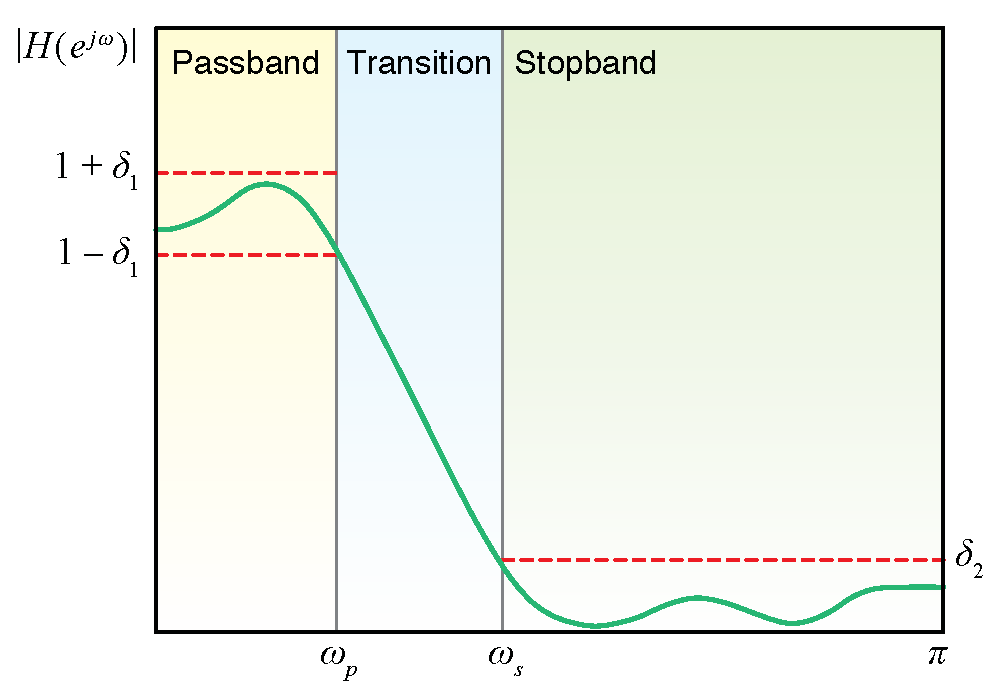
\includegraphics
        [width=\columnwidth]
    	{figures/pdf/figure4.pdf} 
    \caption{Specification for effective frequency response
    for the case of low-pass filter. (the discrete-time system).}
\end{figure}

A Type I Chebyshev filter has an equiripple characteristic in the passband and varies monotonically in the stopband. An elliptic filter is equiripple in both the passband and the stopband. All these approximation methods yield digital filters with non-constant group delay or, equivalently, non-linear phase. The greatest deviation from the constant group delay occurs, in all, cases at the edge of the passband or in the transition band. If phase linearity is not an issue, then elliptic approximation yields the lowest order system function, and therefore elliptic filters will generally require the least computation to implement a given filter specification \citep{Oppenheim_1989}. Altogether, the primary advantage of IIR filters over FIR filters is that the former typically meet a given set of specifications with a much lower filter order than its corresponding FIR filter. Although IIR filters have nonlinear phase, data processing using software such as MATLAB is commonly performed at a post-processing stage (offline), and therefore the entire data sequence is available for filtering. This allows one to use non-causal, zero-phase filtering approach by forward and backward filtering (two-pass) the signals (e.g., via the filtfilt function). This process eliminates the nonlinear phase distortion of IIR filters. Here, we adopt this strategy and all of our filters are zero phase. Consequently, we do not address phase variations and concentrate only on amplitude effects.
